\section{Auswertung}
\label{sec:Auswertung}

\subsection{Runder Stab, einseitige Einspannung}
Zunächst soll die Gesamtauslenkung bestimmt werden.
Dafür zieht man die Nullmessung von der Messung mit Gewicht ab.
Außerdem werden die Stellen, an denen der Stab gemessen wurde, in die Formel 
\begin{equation}
  f(x) = Lx^2 - \frac{x^3}{3}
\end{equation}
eingesetzt und dann als x Koordinate für den Plot verwendet.
Die Ergebnisse sind in Tabelle \ref{tab:runderstabeinseitig} aufgetragen.

Aus der Ausgleichrechnung für den Plot in Abbildung \ref{fig:plot1} mit dem Ansatz
\begin{equation*}
  y(x) = a + b \cdot x
\end{equation*}
gehen die Parameter
\begin{align*}
  a &= 0.0380 ± 0.0004 \frac{1}{\unit{\meter\squared}} & \text{und}& & b&= (0.1248 ± 0.0193) \cdot 10^{-3} \unit\meter\\
\end{align*}
hervor. Nun wird diese Gerade mit der Formel für das Elastizitätsmodul $E$ in (\ref{tbd}) verglichen, wobei für $I$ nach (\ref{eq:FlTreagKreis})
\begin{equation*}
  I = \frac{R^4 \pi}{2} = \frac{0.005^4 \pi}{2}
\end{equation*}
und es gilt
\begin{equation*}
  E = \frac{m \cdot g} {2 \cdot I \cdot a} = (108.4 \pm 1.1) 10^9 \frac{\unit\newton}{\unit\meter^2} \text{ .}
\end{equation*}

Dieser Wert wird mit dem Literaturwert {\cite{demtroeder1}}
\begin{equation*}
  E_\text{Lit} = 125 \cdot 10^9 \frac{\unit\newton}{\unit\meter^2}
\end{equation*}
von Kupfer verglichen. Dabei ergibt sich eine Abweichung von
\begin{equation*}
  \increment E = \left|\frac{108.4 - 125}{125}\right| \cdot 100 = 13.28 \%
\end{equation*}
vom Theoriewert.

\begin{table}[H]
  \centering
  \caption{Messwerte der Auslenkung des runden Stabes bei einseitiger Einspannung.}
  \label{tab:runderstabeinseitig}
  \begin{tabular}{c c c c c}
    \toprule
      $x / 10 ^{-3} \unit\meter$ &  $D_0 (x) / 10^{-3} \unit\meter$ &
        $D_m (x) / 10^{-3} \unit\meter$ & $D(x) / 10^{-3} \unit\meter$ & $(Lx^2 - \frac{x^3}{3}) / 10^{-3} \unit\meter$\\
    \midrule
       30.000 & 0.000 & 0.040 & 0.040 &   0.522 \\
       50.000 & 0.020 & 0.200 & 0.180 &   1.433 \\
       70.000 & 0.006 & 0.280 & 0.274 &   2.777 \\
       90.000 & 0.120 & 0.350 & 0.230 &   4.536 \\
      110.000 & 0.200 & 0.530 & 0.330 &   6.695 \\
      130.000 & 0.290 & 0.715 & 0.425 &   9.239 \\
      150.000 & 0.380 & 0.980 & 0.600 &  12.150 \\
      170.000 & 0.495 & 1.200 & 0.705 &  15.413 \\
      190.000 & 0.640 & 1.460 & 0.820 &  19.013 \\
      210.000 & 0.700 & 1.710 & 1.010 &  22.932 \\
      230.000 & 0.830 & 2.010 & 1.180 &  27.155 \\
      250.000 & 0.920 & 2.310 & 1.390 &  31.667 \\
      270.000 & 1.070 & 2.610 & 1.540 &  36.450 \\
      290.000 & 1.160 & 2.950 & 1.790 &  41.489 \\
      310.000 & 1.350 & 3.300 & 1.950 &  46.769 \\
      330.000 & 1.440 & 3.630 & 2.190 &  52.272 \\
      350.000 & 1.610 & 3.980 & 2.370 &  57.983 \\
      370.000 & 1.765 & 4.350 & 2.585 &  63.887 \\
      390.000 & 1.925 & 4.710 & 2.785 &  69.966 \\
      410.000 & 2.090 & 5.120 & 3.030 &  76.205 \\
      430.000 & 2.280 & 5.510 & 3.230 &  82.589 \\
      450.000 & 2.430 & 5.910 & 3.480 &  89.100 \\
      470.000 & 2.540 & 6.340 & 3.800 &  95.723 \\
      490.000 & 2.830 & 6.690 & 3.860 & 102.443 \\
    \bottomrule
    \end{tabular}
\end{table}

\begin{figure}[H]
  \centering
  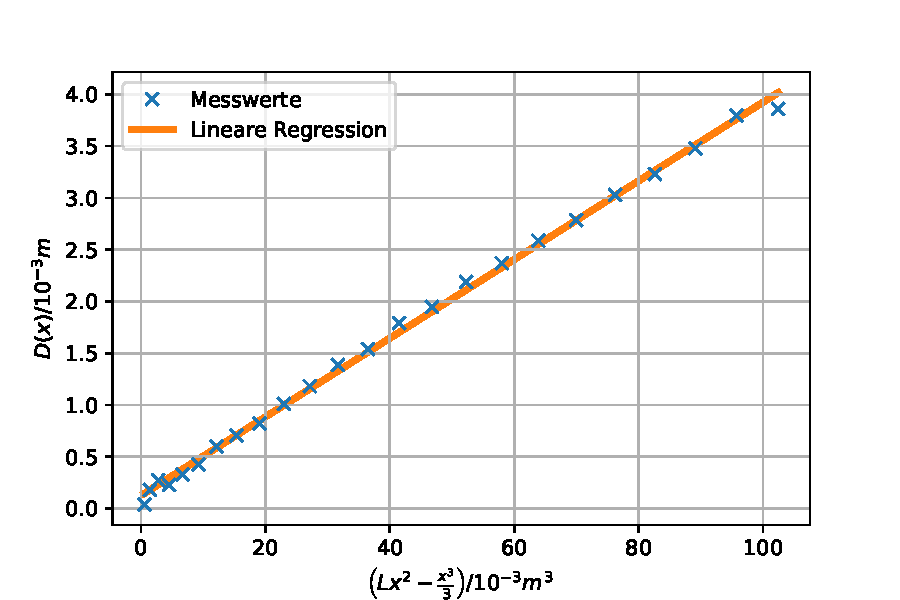
\includegraphics{pictures/Lineare Regression1.pdf}
  \caption{Plot des runden, einseitig eingespannten Stabes gegen die lin. Regression.}
  \label{fig:plot1}
\end{figure}

\subsection{Eckiger Stab, einseitige Einspannung}

Für den eckigen Stab wird analog vorgangen.
Die Messwerte für diese Messung sind in Tabelle \ref{tab:eckigerstabeinseitig} zu finden.
Die Ausgleichsgerade $y(x) = a \cdot x + b$ in Abbildung \ref{fig:plot2} hat die Parameter
\begin{align*}
  a &= 0.0254 ± 0.0003 \frac{1}{\unit{\meter\squared}} & \text{und}& & b&= (0.0401 ± 0.0138) \cdot 10^{-3} \unit\meter \text{ .} \\
\end{align*}
Das Flächenträgheitsmoment wird nach Formel (\ref{eq:FlTreagKreis}) bestimmt und liefert mit Höhe $H = 0.01 \unit\meter$
\begin{equation*}
  I_\text{Quadrat} = \frac{h^4} {12} = \frac{0.01^4} {12} \text{ .}
\end{equation*}
Nun kann das Elastizitätsmodul berechnet werden zu
\begin{equation*}
  E = (124.3 \pm 1.5) \cdot 10^{9} \text{ .}
\end{equation*}
Vergleicht man das mit dem Literaturwert ergibt sich eine Abweichung von
\begin{equation*}
  \increment E = \left|\frac{124.3 - 125}{125}\right| \cdot 100 = 0.56 \% \text{ .}
\end{equation*}




\begin{table}[H]
  \centering
  \caption{Messwerte der Auslenkung des eckigen Stabes bei einseitiger Einspannung.}
  \label{tab:eckigerstabeinseitig}
  \begin{tabular}{c c c c c}
    \toprule
    $x / 10 ^{-3} \unit\meter$ &  $D_0 (x) / 10^{-3} \unit\meter$ &
    $D_m (x) / 10^{-3} \unit\meter$ & $D(x) / 10^{-3} \unit\meter$ & $(Lx^2 - \frac{x^3}{3}) / 10^{-3} \unit\meter$\\
    \midrule
    30.000 & 0.000 & 0.030 & 0.030 &   0.533 \\
    50.000 & 0.010 & 0.040 & 0.030 &   1.463 \\
    70.000 & 0.042 & 0.085 & 0.043 &   2.835 \\
    90.000 & 0.040 & 0.160 & 0.120 &   4.633 \\
    110.000 & 0.050 & 0.270 & 0.220 &   6.841 \\
    130.000 & 0.095 & 0.370 & 0.275 &   9.441 \\
    150.000 & 0.130 & 0.500 & 0.370 &  12.420 \\
    170.000 & 0.200 & 0.650 & 0.450 &  15.760 \\
    190.000 & 0.290 & 0.815 & 0.525 &  19.446 \\
    210.000 & 0.310 & 0.950 & 0.640 &  23.461 \\
    230.000 & 0.390 & 1.160 & 0.770 &  27.790 \\
    250.000 & 0.490 & 1.370 & 0.880 &  32.417 \\
    270.000 & 0.580 & 1.560 & 0.980 &  37.325 \\
    290.000 & 0.610 & 1.760 & 1.150 &  42.499 \\
    310.000 & 0.620 & 1.965 & 1.345 &  47.922 \\
    330.000 & 0.730 & 2.180 & 1.450 &  53.579 \\
    350.000 & 0.800 & 2.380 & 1.580 &  59.453 \\
    370.000 & 0.880 & 2.620 & 1.740 &  65.529 \\
    390.000 & 1.000 & 2.880 & 1.880 &  71.791 \\
    410.000 & 1.100 & 3.150 & 2.050 &  78.223 \\
    430.000 & 1.210 & 3.380 & 2.170 &  84.807 \\
    450.000 & 1.300 & 3.640 & 2.340 &  91.530 \\
    470.000 & 1.385 & 3.905 & 2.520 &  98.374 \\
    490.000 & 1.450 & 4.050 & 2.600 & 105.324 \\
    \bottomrule
    \end{tabular}
\end{table}

\begin{figure}[H]
  \centering
  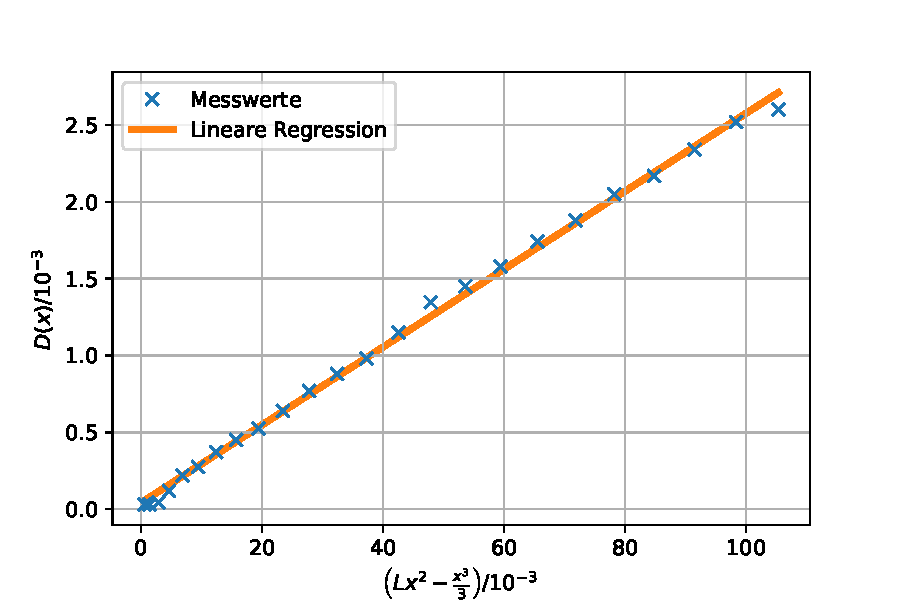
\includegraphics{pictures/Lineare Regression2.pdf}
  \caption{Plot des eckigen, einseitig eingespannten Stabes gegen die lin. Regression.}
  \label{fig:plot2}
\end{figure}


\subsection{Runder Stab, beidseitige Einspannung}

Für die beidseitige Einspannung erhält man die Werte
\begin{align*}
  a &= 0.0036 ± 0.0002 \frac{1}{\unit{\meter\squared}} & \text{und}& & b&= (0.2068 ± 0.0283) \cdot 10^{-3} \unit\meter \text{ .} \\
\end{align*}
Da es sich nun um eine beidseitige Einspannung handelt, muss die Formel (\ref{tbd}) angewendet werden.
Somit wird $E$ zu
\begin{equation*}
  E = \frac{m_\text{angehängt} \cdot g}{48 \cdot I \cdot a} = (180 \pm 10) \cdot 10^{9}
\end{equation*}
bestimmt. Die Abweichung beträgt somit
\begin{equation*}
  \increment E = \left|\frac{180 - 125}{125}\right| \cdot 100 = 44 \% \text{ .}
\end{equation*}

\begin{table}[H]
  \centering
  \caption{Messwerte der Auslenkung des runden Stabes bei beidseitiger Einspannung.}
  \label{tab:runderstabbeidseitig}
  \begin{tabular}{c c c c c}
    \toprule
    $x / 10 ^{-3} \unit\meter$ &  $D_0 (x) / 10^{-3} \unit\meter$ &
    $D_m (x) / 10^{-3} \unit\meter$ & $D(x) / 10^{-3} \unit\meter$ & $(3L^2x - 4x^3) / 10^{-3} \unit\meter$\\
    \midrule
    30.000 & 0.000 & 0.320 & 0.320 &  31.221 \\
    50.000 & 0.120 & 0.570 & 0.450 &  51.715 \\
    70.000 & 0.240 & 0.770 & 0.530 &  71.729 \\
    90.000 & 0.400 & 0.960 & 0.560 &  91.071 \\
    110.000 & 0.530 & 1.170 & 0.640 & 109.549 \\
    130.000 & 0.640 & 1.360 & 0.720 & 126.971 \\
    150.000 & 0.720 & 1.520 & 0.800 & 143.145 \\
    170.000 & 0.820 & 1.680 & 0.860 & 157.879 \\
    190.000 & 0.910 & 1.810 & 0.900 & 170.981 \\
    210.000 & 0.960 & 1.860 & 0.900 & 182.259 \\
    230.000 & 1.010 & 1.960 & 0.950 & 191.521 \\
    250.000 & 1.060 & 2.030 & 0.970 & 198.575 \\
    270.000 & 1.090 & 2.060 & 0.970 & 203.229 \\
    285.000 & 0.180 & 1.140 & 0.960 & 205.029 \\
    305.000 & 0.200 & 1.130 & 0.930 & 205.021 \\
    325.000 & 0.200 & 1.100 & 0.900 & 202.085 \\
    345.000 & 0.190 & 1.050 & 0.860 & 196.029 \\
    365.000 & 0.180 & 0.980 & 0.800 & 186.661 \\
    385.000 & 0.170 & 0.910 & 0.740 & 173.789 \\
    405.000 & 0.160 & 0.830 & 0.670 & 157.221 \\
    425.000 & 0.150 & 0.740 & 0.590 & 136.765 \\
    445.000 & 0.120 & 0.630 & 0.510 & 112.229 \\
    465.000 & 0.100 & 0.520 & 0.420 &  83.421 \\
    485.000 & 0.100 & 0.460 & 0.360 &  50.149 \\
    505.000 & 0.060 & 0.270 & 0.210 &  12.221 \\
    525.000 & 0.000 & 0.120 & 0.120 & -30.555 \\
    \bottomrule
    \end{tabular}
\end{table}

\begin{figure}[H]
  \centering
  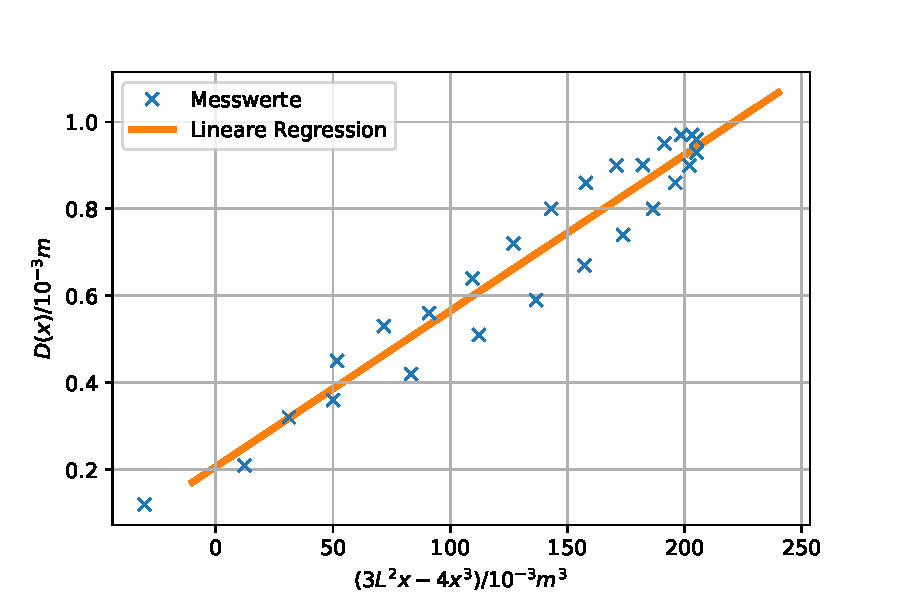
\includegraphics{pictures/Lineare Regression3.pdf}
  \caption{Plot des runden, beidseitig eingespannten Stabes gegen die lin. Regression.}
  \label{fig:plot3}
\end{figure}


\subsection{Eckiger Stab, beidseitige Einspannung}

Es ergeben sich die Werte 
\begin{align*}
  a &= 0.0032 ± 0.0006 \frac{1}{\unit{\meter\squared}} & \text{und}& & b&= (-0.2266 ± 0.0971) \cdot 10^{-3} \unit\meter \text{ .} \\
\end{align*}
Nun kann das Elastizitätsmodul berechnet werden. Es gilt
\begin{equation*}
  E = \frac{m_\text{angehängt} \cdot g}{48 \cdot I \cdot a} = (119 \pm 22) \cdot 10^{9} \text{ .}
\end{equation*}
Die Abweichung beträgt
\begin{equation*}
  \increment E = \left|\frac{119 - 125}{125}\right| \cdot 100 = 4.8 \% \text{ .}
\end{equation*}

\begin{table}[H]
  \centering
  \caption{Messwerte der Auslenkung des eckigen Stabes bei beidseitiger Einspannung.}
  \label{tab:eckigerstabbeidseitig}
  \begin{tabular}{c c c c c}
    \toprule
    $x / 10 ^{-3} \unit\meter$ &  $D_0 (x) / 10^{-3} \unit\meter$ &
    $D_m (x) / 10^{-3} \unit\meter$ & $D(x) / 10^{-3} \unit\meter$ & $(3L^2x - 4x^3) / 10^{-3} \unit\meter$\\
    \midrule
    30.000 & 0.000 & 0.260 &  0.260 &  32.508 \\
    50.000 & 0.030 & 0.280 &  0.250 &  53.861 \\
    70.000 & 0.070 & 0.280 &  0.210 &  74.733 \\
    90.000 & 0.110 & 0.300 &  0.190 &  94.933 \\
    110.000 & 0.160 & 0.300 &  0.140 & 114.269 \\
    130.000 & 0.220 & 0.320 &  0.100 & 132.550 \\
    150.000 & 0.270 & 0.270 &  0.000 & 149.582 \\
    170.000 & 0.310 & 0.290 & -0.020 & 165.174 \\
    190.000 & 0.360 & 0.280 & -0.080 & 179.134 \\
    210.000 & 0.440 & 0.210 & -0.230 & 191.271 \\
    230.000 & 0.490 & 0.130 & -0.360 & 201.391 \\
    250.000 & 0.550 & 0.120 & -0.430 & 209.303 \\
    270.000 & 0.630 & 0.040 & -0.590 & 214.815 \\
    295.000 & 0.900 & 1.500 &  0.600 & 218.038 \\
    305.000 & 0.850 & 1.460 &  0.610 & 218.109 \\
    325.000 & 0.800 & 1.400 &  0.600 & 216.031 \\
    345.000 & 0.740 & 1.300 &  0.560 & 210.834 \\
    365.000 & 0.630 & 1.170 &  0.540 & 202.324 \\
    385.000 & 0.550 & 1.050 &  0.500 & 190.310 \\
    405.000 & 0.500 & 0.920 &  0.420 & 174.600 \\
    425.000 & 0.400 & 0.810 &  0.410 & 155.003 \\
    445.000 & 0.340 & 0.680 &  0.340 & 131.325 \\
    465.000 & 0.250 & 0.530 &  0.280 & 103.375 \\
    485.000 & 0.240 & 0.430 &  0.190 &  70.961 \\
    505.000 & 0.110 & 0.300 &  0.190 &  33.892 \\
    525.000 & 0.000 & 0.110 &  0.110 &  -8.026 \\
    \bottomrule
    \end{tabular}
\end{table}

\begin{figure}[H]
  \centering
  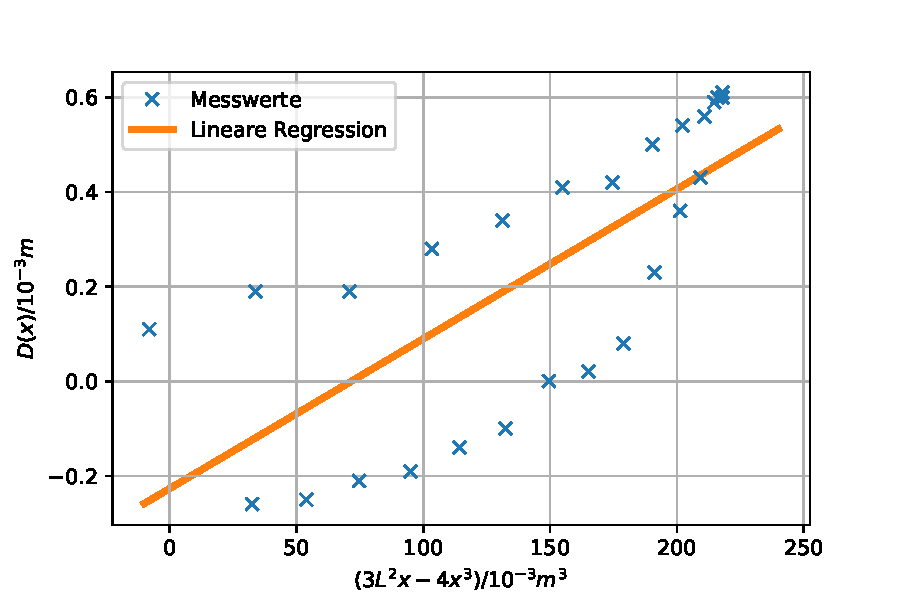
\includegraphics{pictures/Lineare Regression4.pdf}
  \caption{Plot des eckigen, beidseitig eingespannten Stabes.}
  \label{fig:plot3}
\end{figure}